\documentclass{article}
%\VignetteIndexEntry{Using rnbn}
\usepackage{hyperref}
\usepackage{graphicx}
\usepackage{array}

% bibliography style
\usepackage[sectionbib,round]{natbib}
\bibliographystyle{mybst}

\usepackage{Sweave}
\begin{document}
\Sconcordance{concordance:rnbn.tex:rnbn.Rnw:%
1 10 1 1 0 114 1 1 2 1 0 1 1 1 2 7 0 1 2 40 1 1 2 1 0 1 3 13 0 1 2 3 1 %
1 3 2 0 1 2 7 0 1 2 123 1}


\title{Extract data from the NBN Gateway into R}
\author{Stuart Ball, JNCC.}
\date\today
\maketitle
\section{Introduction}
The National Biodiversity Network (NBN) is an on-line repository for biodiversity
data from the UK. At the time of writing, it contained over 85 million species
records in over 800 datasets. Data can be accessed via web-services provided by
the Gateway web-site (for documentation see \url{http://data.nbn.org.uk/Documentation/Web\textunderscore Services/}).

This package provides methods to get species records and other supporting
information from the NBN Gateway. The functions fall into three tiers:
\begin{description}
  \item[Low level functions] to prepare the ground
  \begin{description}
    \item [makenbnurl] constructs a URL to call a service from the supplied
    parameters (and check they are correct!)
    \item [runnbnurl] run the URL and return the JSON object obtained in response
    to the web-service call in the form of an R list structure
  \end{description}
  \item[Functions that access a particular service] and return a JSON object
  \begin{description}
      \item[getOccurrences] get occurrences for a particular taxon or list of
      taxa. Returns a data.frame containing the occurrences. Optionally, the
      datasets from which observations are to be extracted and a start and end
      year can also be specified.
      \item[getTaxon] get information about a particular taxon given its Taxon
      Version Key (TVK).
      \item[getFeature] get information about a "feature" (a location at which
      occurrences have been recorded) given its featureID.
  \end{description}
  \item[High levels functions] that manipulate the returned data for
  a particular purpose
  \begin{description}
      \item[getSDMdata] get the necessary occurrence information for one or
      more species to run a Species Distribution Model. This returns a 
      data.frame containing the x,y coordinates of occurrences, which 
      is the format required by various R modelling packages (such as dismo),
      but the information can also be saved to a CSV file for use with external
      modelling software such as maxent.
      \item[getFrescaloData] get the necessary data to run Mark Hill's Frescalo
      method to estimate species trends.
  \end{description}
\end{description}

Some other utility functions are provided which manipulate grid reference and
date information returned by the NBN Gateway:
\begin{description}
  \item[gridRef] takes a grid reference string (OSGB or OSNI) and extracts grid
  references at other precisions. For example, extract 10km square grid refs
  from the grid references returned from the Gateway.
  \item[gridCoords] takes a grid reference string (OSGB or OSNI) and calculates
  the x,y coordinates of the bottom, left-hand corner of the grid square.
  \item[datePart] takes the vague date information, returned in three fields
  (startDate, endDate and dateTypeKey) from the NBN Gateway and extracts elements
  of the date like the year or week, whilst properly taking into account the
  type of vague date. 
\end{description}

\section{Getting species occurrence records}
The \texttt{getOccurrences} function gets a data.frame of species occurrence records from
the NBN Gateway. Columns include the name and TVK of the species and the date
and location of the observation as a minimum, and may include other columns
depending what has been submitted by the data providers and what access they
allow.

The minimum information required to request species occurrences from the NBN
Gateway is the Taxon Version Key (TVK) of your target species. This is a 
16-character string of (usually, upper-case) letters and numbers. For example,
``NBNSYS0000007111''.

TVKs can be found by searching for a species on the NBN Gateway. At the time of
writing, there is no web-service to do this, although it should be available
soon. Consequently, this will have to be done manually.

\begin{enumerate}
\begin{tabular}{ p{0.3\textwidth} m{0.7\textwidth} }
  \item On the NBN Gateway home page \url{http://data.nbn.org.uk/}, type the
  name of the species (``Tropidia scita'' in the example) in the ``Search for
  species or sites'' box and press Return or click the ``search'' button.
  &
  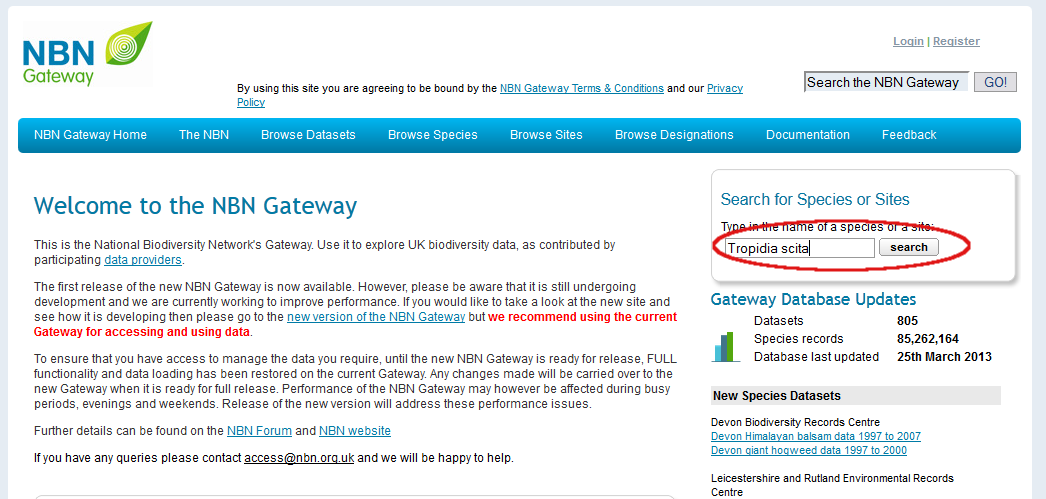
\includegraphics[width=0.66\textwidth]{NBN_search.png}
  \\
  \item Hopefully, one or more matches will be found. Click the ``Taxonomy and
  designation information for \ldots'' link.
  &
  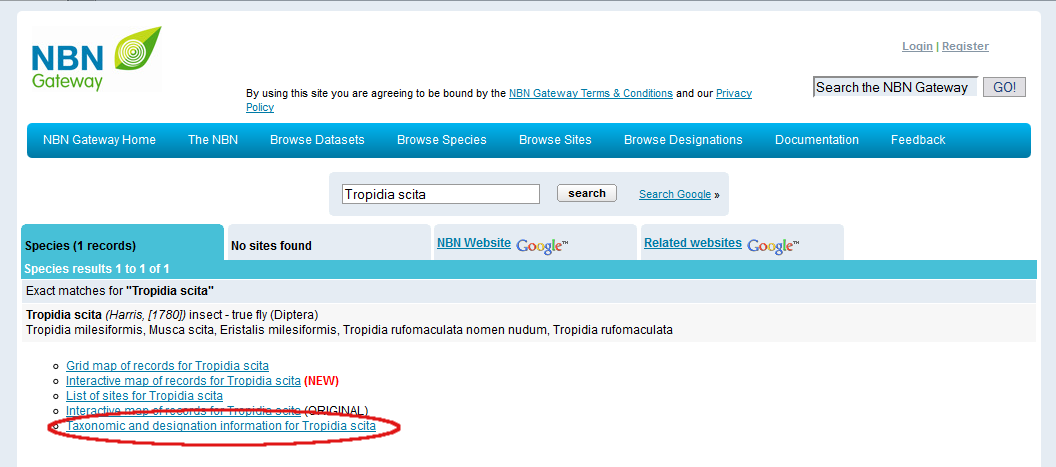
\includegraphics[width=0.66\textwidth]{NBN_search_result.png}
  \\
  \item This will display the ``NBN Taxonomic and Designation Information'' page
  for the species. The TVK is shown below the name of the species.
  &
  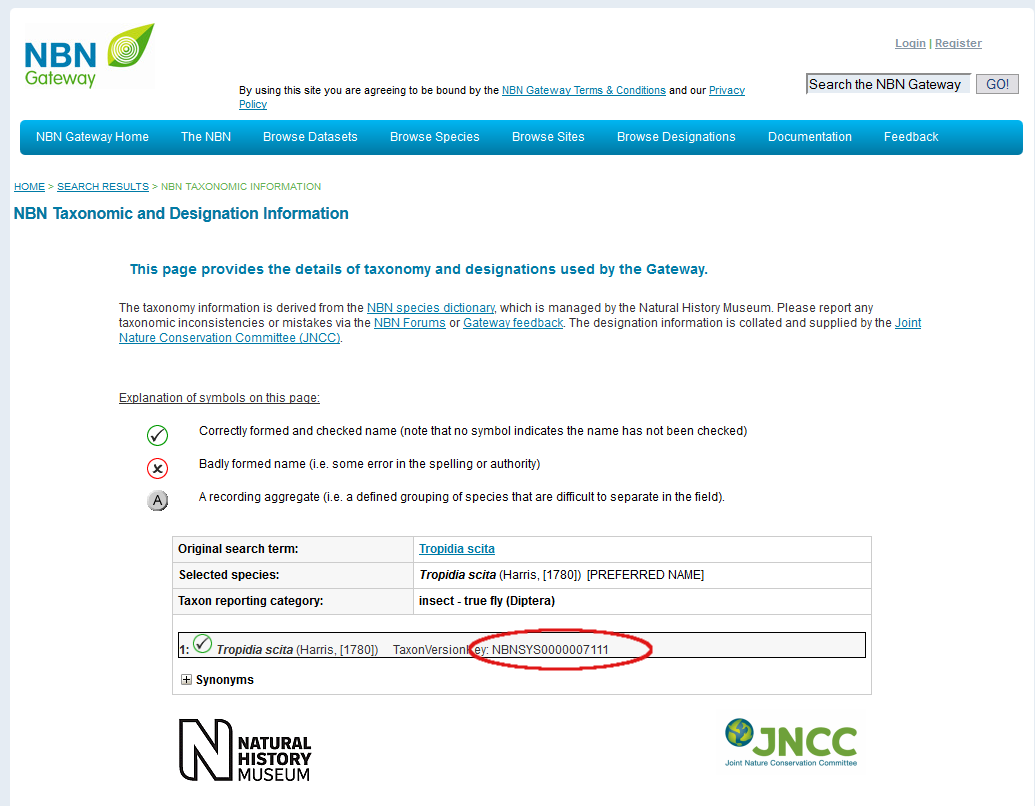
\includegraphics[width=0.66\textwidth]{NBN_species_taxonomy.png}
  \\
\end{tabular}
\end{enumerate}

For example, the following example will get all publicly available observations
of \emph{Tropidia scita} from all datasets and for any date and lists selected
columns for the first 10 rows:

\begin{Schunk}
\begin{Sinput}
> library(rnbn)
> dt <- getOccurrences(tvks="NBNSYS0000007111")
> dt[1:10,c("observationID","pTaxonName","location","startDate","endDate",
+           "dateTypekey")]
\end{Sinput}
\begin{Soutput}
   observationID     pTaxonName location  startDate    endDate dateTypekey
1         454832 Tropidia scita TL531621 2006-06-29 2006-06-29          D 
2         455412 Tropidia scita TL529622 1986-09-01 1986-09-01          D 
3         455546 Tropidia scita TL531628 1960-01-01 1960-12-31          Y 
4         659031 Tropidia scita   SD4869 1999-06-18 1999-06-18          D 
5         661408 Tropidia scita   SD5152 1999-06-16 1999-06-16          D 
6         662641 Tropidia scita   SD4875 1999-06-13 1999-06-13          D 
7         663098 Tropidia scita   SD5151 1999-06-16 1999-06-16          D 
8         813629 Tropidia scita   SU3738 1985-07-01 1985-07-01          D 
9         813889 Tropidia scita   SH6172 1987-07-09 1987-07-09          D 
10        824086 Tropidia scita    SK60H 1973-01-01 1973-12-31          Y 
\end{Soutput}
\end{Schunk}

Occurrences for more than one species can be obtained by  passing a list of
TVKs, e.g. 
\begin{verbatim}
tvks=c("NBNSYS0000007111","NBNSYS0000007073")
\end{verbatim}

Observations can be filtered so that they come only from datasets you trust
by passing one or more dataset keys to the datasets parameter. A list
of datasets can be passed in a way similar to a list of species keys. e.g.
\begin{verbatim}
datasets= c("SGB00001","GA000483","GA000152","GA000306")
\end{verbatim}

Dataset IDs are 8-character strings of upper-case letters and numbers. Like
TVKs, at present, you will need to manually look them up from the NBN Gateway 
web-site as follows:

\begin{enumerate}
\begin{tabular}{ m{0.3\textwidth} m{0.7\textwidth} }
  \item On the NBN Gateway home page \url{http://data.nbn.org.uk/}, click the
  ``Browse Datasets'' button in the menu bar at the top of the page and then
  click the ``All species datasets'' link.
  &
  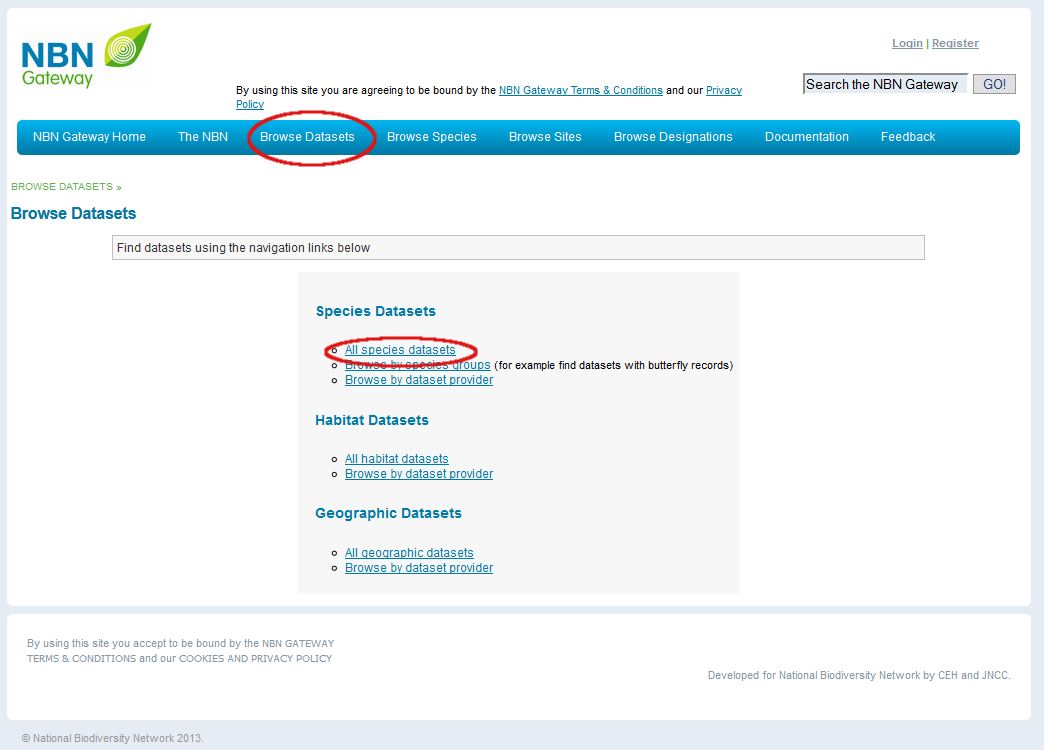
\includegraphics[width=0.66\textwidth]{NBN_datasets.png}
  \\
  \item Find the dataset you are interested in by scrolling through the 
  alphabetic list of datasets that appears. When you find the one you want,
  click on its name.
  &
  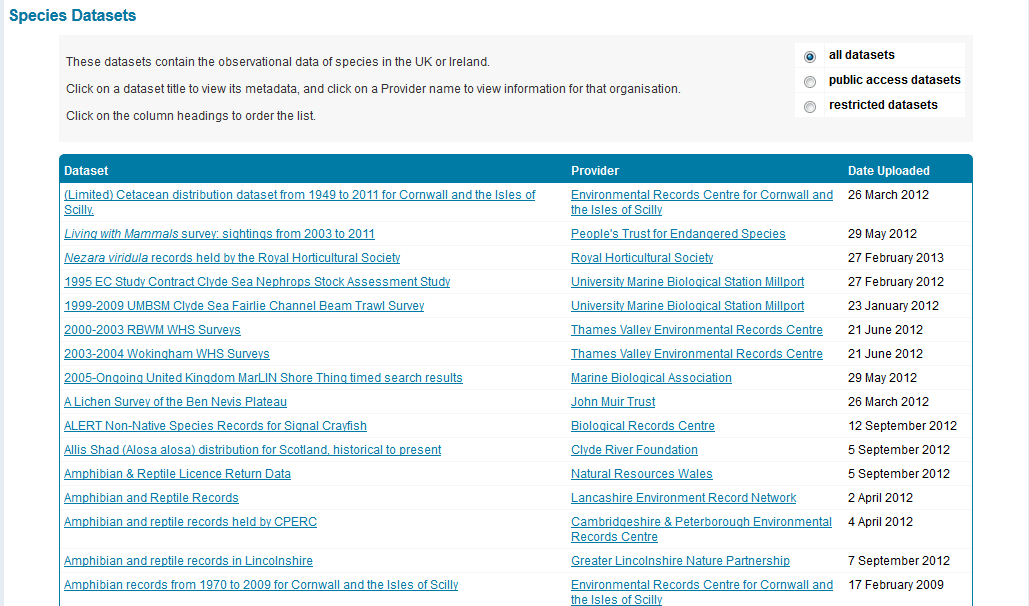
\includegraphics[width=0.66\textwidth]{NBN_datasets_list.png}
  \\
  \item This will display a page of metadata about the selected dataset. The
  dataset key is near the bottom of the first section ``Dataset Details''
  and just before the ``Dataset Use'' section starts.
  &
  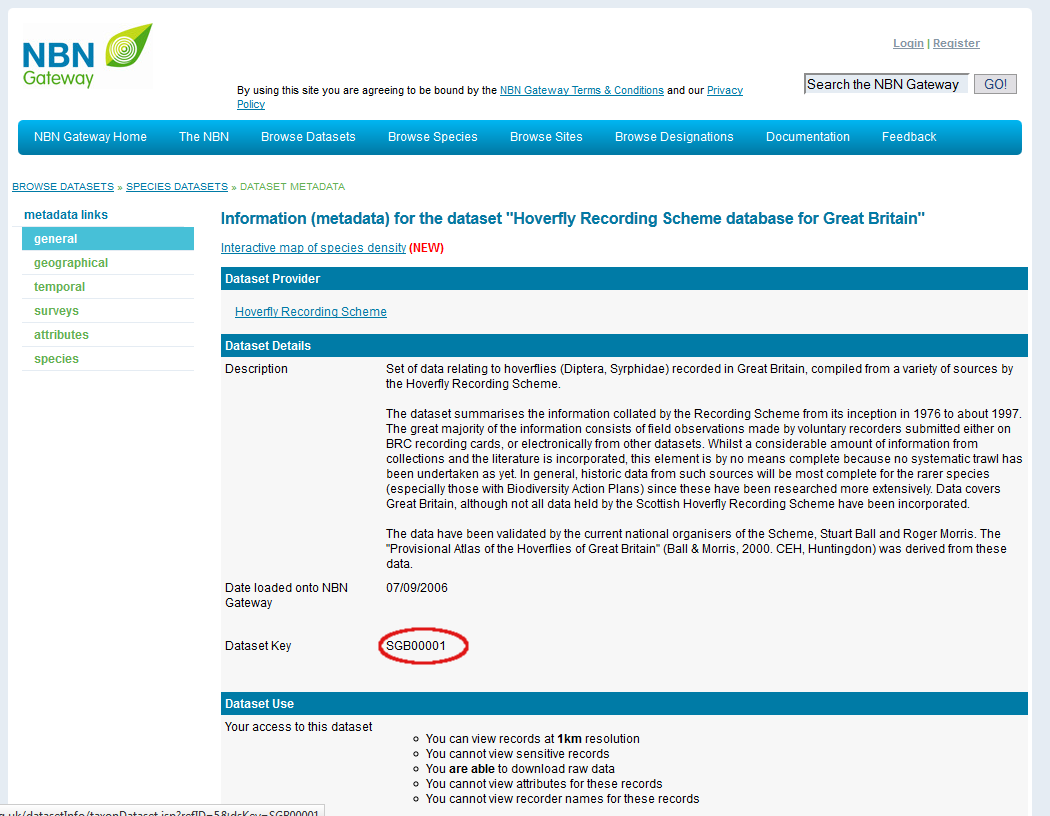
\includegraphics[width=0.66\textwidth]{NBN_dataset_details.png}
  \\
\end{tabular}
\end{enumerate}

The range of dates for which you want to extract data can also be specified 
using the \texttt{startYear} and/or \texttt{endYear} parameters:

\begin{Schunk}
\begin{Sinput}
> dt <- getOccurrences(tvks="NBNSYS0000007111", datasets="SGB00001", 
+                      startYear=1990, endYear=2006)
> dt[1:10,c("observationID","pTaxonName","location","startDate","endDate",
+           "dateTypekey")]
\end{Sinput}
\begin{Soutput}
   observationID     pTaxonName location  startDate    endDate dateTypekey
1       17301681 Tropidia scita   SU3614 1992-01-01 1992-12-31          Y 
2       17302534 Tropidia scita   NR6822 2005-06-17 2005-06-17          D 
3       17306319 Tropidia scita   TG0111 1993-07-06 1993-07-06          D 
4       17306359 Tropidia scita   TM3991 1993-07-07 1993-07-07          D 
5       17306370 Tropidia scita   TM5093 1993-07-07 1993-07-07          D 
6       17306338 Tropidia scita   TG4222 1993-07-05 1993-07-05          D 
7       17318254 Tropidia scita   SD5152 1999-06-16 1999-06-16          D 
8       17321928 Tropidia scita   TF0270 2002-06-20 2002-06-20          D 
9       17321987 Tropidia scita   TF1417 1998-06-20 1998-06-20          D 
10      17321971 Tropidia scita   TF1218 1998-07-02 1998-07-02          D 
\end{Soutput}
\end{Schunk}

\section{Getting data for Species Distribution Models and Frescalo}

\subsection{\texttt{getSDMdata}}
The function \texttt{getSDMdata} gets the data required to fit a Species 
Distribution Mode for one or more species from the NBN Gateway. One element
required by many
modelling methods consists of the coordinates of the locations at which a 
species has been observed. This is often supplied in the form of a CSV file with
either the x,y coordinates for a particular species in two columns or, if the
method can fit a sequence of species in one run, then species name,x,y in three
columns. If modelling is being done via an R package such as dismo 
(\cite{Hijmans2013}), then the coordinates are generally supplied as x,y columns
in a matrix or data.frame. These functions assumes that you are fitting a model
Using coordinates of the National Grid for either GB or Ireland.

\subsection{\texttt{getFrescaloData}}
Mark Hill's Frescalo method (\cite{Hill2012}) calculates trends in the frequency
of a species over time. It attempts to correct the frequency with which a
species has been recorded in a series of time periods using the total amount
of recording. This is done by identifying the commonest species in a 
neighbourhood around a given location and then quantifying the recording effort
in terms of the proportion of the commonest species that were recorded in the
neighbourhood. The basic assumption is that the more recording, the greater the
proportion of commoner species that will be discovered. One of the inputs 
required is a set of observations consisting of unique combinations of location,
species and time period. \texttt{getFrescaloData} extracts this information from
observations obtained from the NBN Gateway and writes them to a file in a
suitable format for Frescalo. Grid squares are used to provide the locations.

\subsection{Specifying species}
The format of the species parameter is the same for \texttt{getSDMdata},
and \texttt{getFrescaloData}, i.e. a data frame with columns \texttt{tvk} and
\texttt{name}. In general, you will probably specify one or a few species for
\texttt{getSDMdata},
but a list covering a large number of species for \texttt{getFrescaloData}. This is
because the Frescalo method corrects for recording effort using the amount of
recording of common species in the same group. You will therefore need to list
all the species covered, e.g. all the species in a family. This is most 
conveniently done as an external file with a line for each TVK. In preparing this
file, you will also need to consider how the species should be aggregated. There
may be subspecies or named forms where you wish to combine 
the observations under a single name or groups of species which need to be 
aggregated, for example, a recently split group of sibling species. This can be 
achieved by assigning the same entry in the \texttt{name} column to two or 
more entries in the \texttt{tvk} column. 

Example (extracts from a CSV file):
 
\begin{verbatim}
name,tvk
Anasimyia contracta,NBNSYS0000007039
Anasimyia interpuncta,NBNSYS0000007040
Anasimyia lineata,NBNSYS0000007041
...
Platycheirus peltatus agg,NBNSYS0000006879
Platycheirus peltatus agg,NBNSYS0000006886
Platycheirus peltatus agg,NBNSYS0000033188
...
Volucella bombylans,NBNSYS0000007094
Volucella bombylans,NBNSYS0000172195
\end{verbatim}

Here \emph{Platycheirus peltatus} was split into a group of sibling species 
recently, so they are combined as an aggregate named \emph{Platycheirus 
peltatus agg}. Also a form of \emph{Volucella bombylans} is combined under 
the one species name.

If this is stored as \texttt{syrphidae.csv}, it can be loaded as follows:
\begin{verbatim}
sp <- read.csv("/path/syrphidae.csv", as.is=TRUE)
\end{verbatim}

Notice the use of the \texttt{as.is} parameter to prevent strings (in this case,
both the name of species and the TVK are character strings) from being loaded as
factors. 

\subsection{Constructing periods for Frescalo}
Periods are specified as a list with two
items: \texttt{breakYear} and \texttt{plabel}. 

\texttt{breakYear} should contain a
list of year numbers starting at the earliest year you want to include and
finishing with the latest. The number and size of steps is up to you and
periods do not have to be of equal sizes. 

\texttt{plabel} provides the labels
which will be used to identify the periods in the output file. The labels
should be in character format and there should be one less label than the
number of breaks.
 
For example:
\begin{verbatim}
periods <- list()
periods$breakYear <- seq(from=1980, to=2012, by=2)
periods$plabel <- as.character(seq(from=1980, to=2010, by=2))
\end{verbatim}
 
It is believed to be good practice to choose your break points so that
roughly equal numbers of observations fall in each period. Since the amount
of recording (or at least the number of records that have been captured in
databases!) has tended to increase over time for many recording schemes, this
implies that the earlier periods will most likely need to be longer than the
more recent ones.

\subsection{Parallelism}
If the number of species to be covered is 
substantial, this function will take some time (many minutes) to run. The way
that the function works is to find all unique values in the \texttt{name} 
column of the \texttt{species} parameter, then process each of these separately
- using the corresponding \texttt{tvk} entry(s) to call 
\texttt{getOccurrences} and get observations for that species. The
unique location/species name/period combinations are then extracted and
appended to the growing output file. This is ``embarrassingly parallel'' and
scales almost linearly with the number of CPUs available to run it, i.e. a
dual core machine will take only slightly more than half as long as a single
core machine. The \texttt{foreach} package \texttt{\%dopar\%} operator is used.
Therefore you can use any available methods to register a parallel backend
for \texttt{foreach} before calling this function. If no backend is registered
and multiple CPUs are detected, they will be used automatically.

\bibliography{refs}

\end{document}
